\chapter{Analysis}
In this chapter every subcomponent will be part of an experiment in isolation to validate their function. Also, various test setups will be discussed for the purpose of making multi-module experiments in the AFE and control system to evaluate their performance and compatibility.

\section{Validation experiments}
\subsection{Control System}
First, a bitstream was generated with a Pwm generator and AXI interconnect registers. An AXI interconnect register is a method to create GPIO between the FPGA and the Arm processor on the Zynq 7000 SoC using registers that temporarily store GPIO data in the bitstream overlay. A block diagram of the overlay can be seen in \cref{fig:app_fpga_block_diagram} and the JupyterLab notebook can be seen in \cref{fig:app_jupyter_notebook}.

\begin{figure}[htbp]
	\centering
	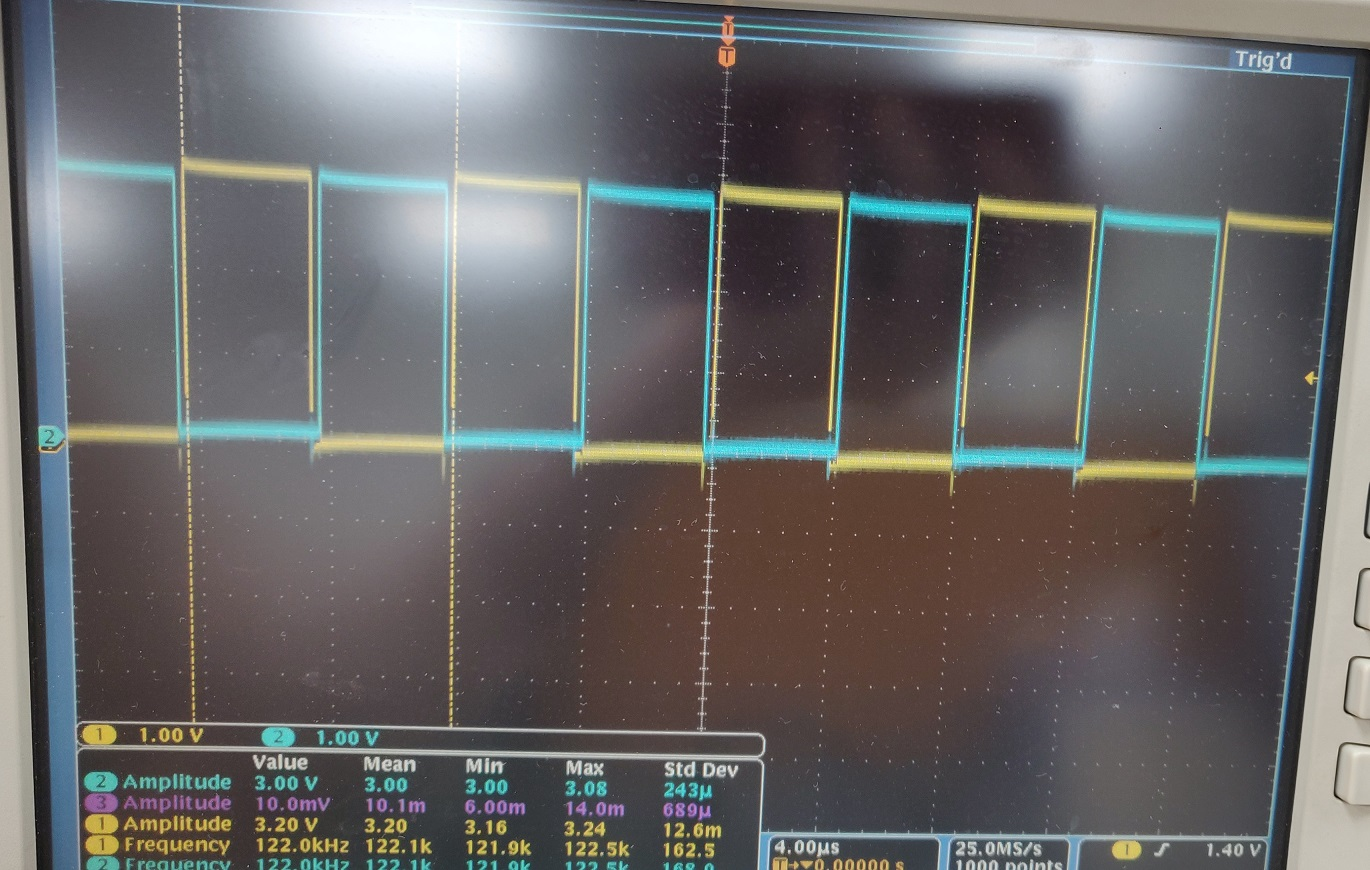
\includegraphics[width=.8\textwidth]{Figures/4_controlsystem_fpga_pwm.png}
	\caption{Complementary PWM output with Pynq Z1 FPGA and JupyterLab notebook}
	\label{fig:4_controlsystem_fpga_pwm}
\end{figure}
A preliminary implementation was implemented in Vivado and JupyterLab for a continuous complementary PWM controller. The resulting measurement can be seen in \cref{fig:4_controlsystem_fpga_pwm} before a clock configuration, which means the frequency corresponded to an arbitrary temporary pulse frequency of \qty{122}{\kilo\hertz}. The design

\subsection{Power Stage}
Seen in \cref{fig:4_transmitter_meas} are actual measured inputs and outputs of the power stage. On the input, there are two complementary \qty{5}{\mega\hertz} signals with varying duty cycle to generate the desired dead time. On the output, we see the rail-to-rail push-pull operation of the \gls{mosfet} half-bridge. The schematic of the transmitter can be found in the appendix in \cref{fig:appendix_md1213db1}. Noticeable noise is observed in the input signal top and base but is negligible for successful operation. Possibly, the noise is due to a cable and adapter setup.
\begin{figure}[htbp]
	\centering
	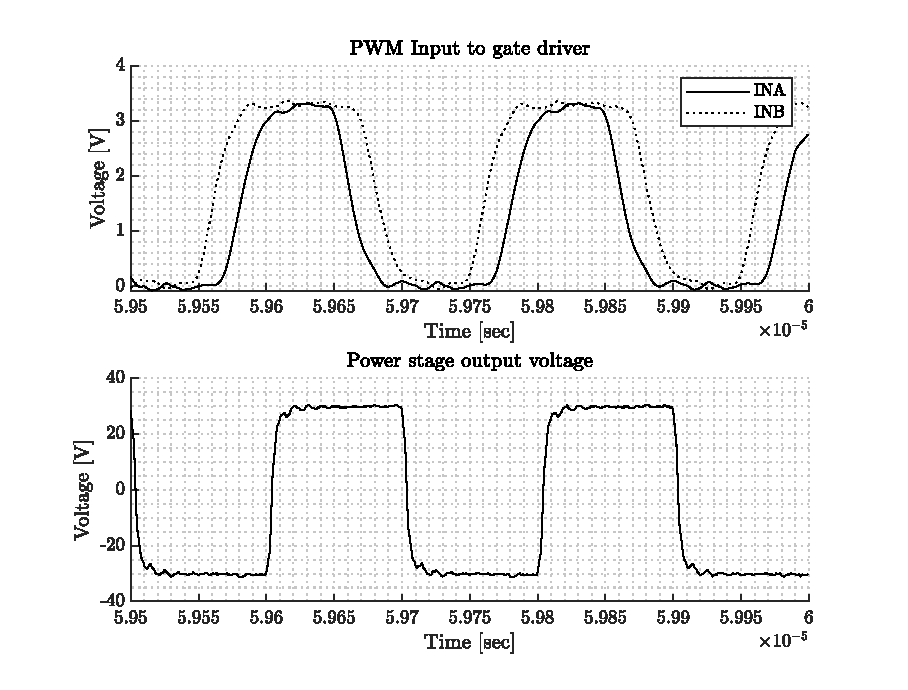
\includegraphics[width=.8\textwidth]{Figures/4_transmitter_pcb_out.eps}
	\caption[Measured input and output of power stage PCB]{Measured input and output of power stage PCB. (Above) Input to gate driver with dead-time (Below) Output of MOSFET half-bridge and the voltage across the load}
	\label{fig:4_transmitter_meas}
\end{figure}

\subsection{Transmit/Receive Switch}
\begin{figure}[htbp]
	\centering
	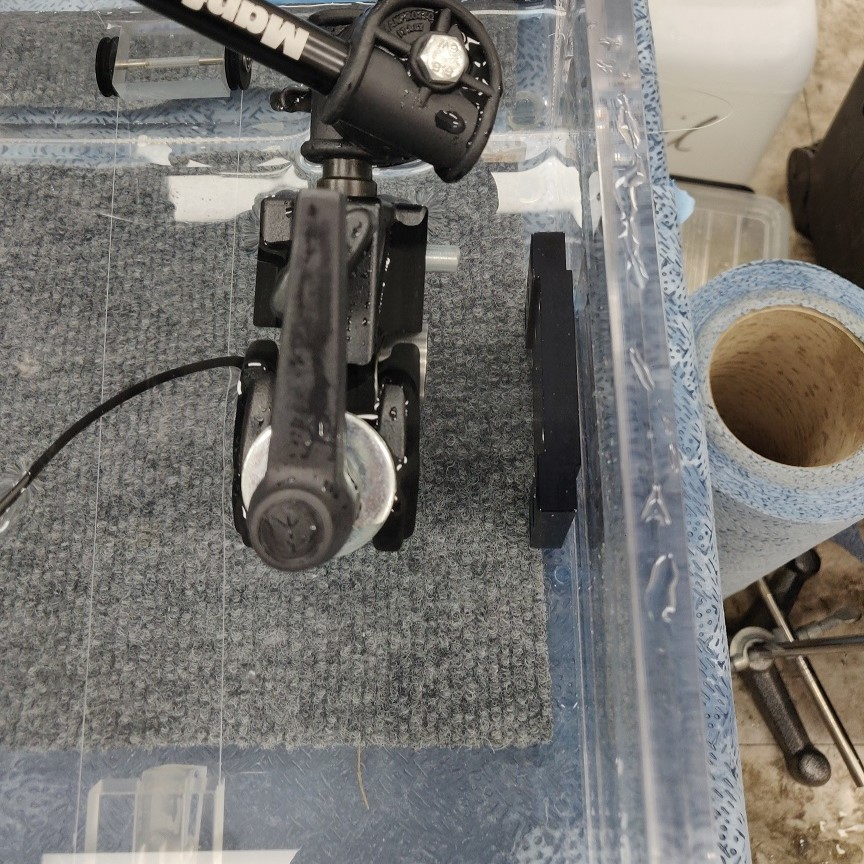
\includegraphics[width=.8\textwidth]{Figures/4_switch_meas_pic.jpg}
	\caption{TX/RX Switch reflection experiment with water tank}
	\label{fig:4_switch_meas_pic}
\end{figure}
For validating the TX/RX switch, an experiment is conducted with a \gls{pzt} transducer, water tank, function generator and an oscilloscope. Using two input signals, $f_{\mathrm{prf}}=\qty{10}{\kilo\hertz}$ switch signal, and $f_{0}=\qty{5}{\mega\hertz}$ burst mode transmit signal, the switch is configured to transmit and receive. A picture of the submerged transducer with a reflector can be seen in \cref{fig:4_switch_meas_pic}. After submerging the transducer in distilled water and measuring on the receiver side of the TX/RX switch, a reflected signal from the tank can be observed in \cref{fig:4_txrx_meas}.
\begin{figure}[htbp]
	\centering
	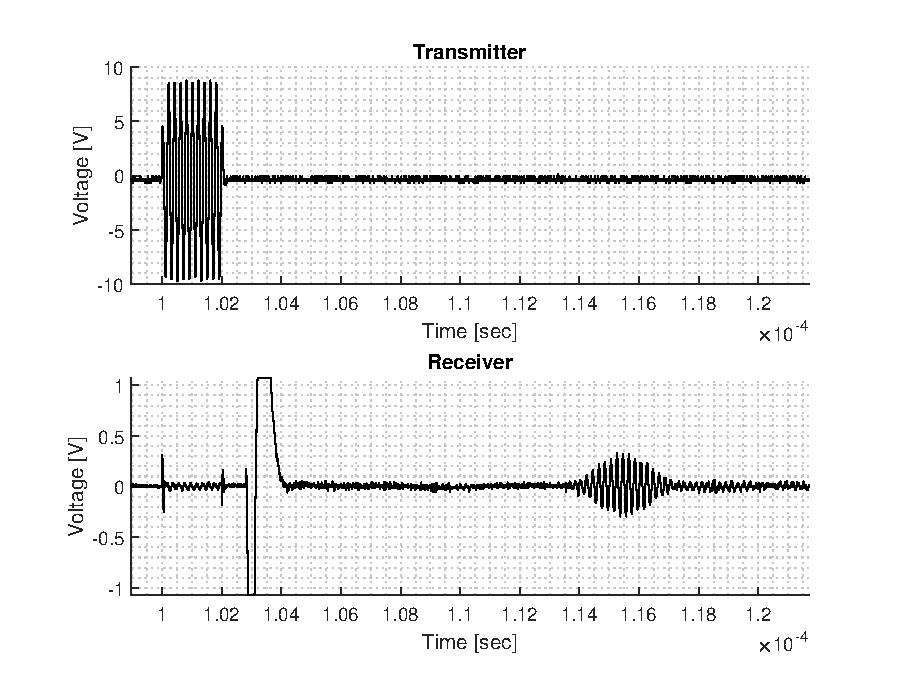
\includegraphics[width=.8\textwidth]{Figures/4_switch_pcb_meas.eps}
	\caption[Measured transmit and receive on Transmit/Receive Switch PCB]{Measured transmit and receive on Transmit/Receive Switch PCB (Above) Measured transmit voltage (Below) Received reflected signal off water tank}
	\label{fig:4_txrx_meas}
\end{figure}

\subsection{Bandpass Filter}
it is desired to validate its frequency response to determine if it functions as desired. To obtain the frequency response, a bode plot of the magnitude and phase is measured from \qty{300}{\kilo\hertz} until \qty{20}{\mega\hertz} using a \gls{vna} in a S21 configuration, meaning a measurement of the output in respect to the input. This measurement determines the difference in magnitude and phase of the output in comparison with the input signal. Observed in \cref{fig:4_bpf_measurement} is the frequency response of the band-pass filter measured on a \gls{vna}. It is noted that the pass band frequencies are mostly as expected with \qty{-0.5}{\decibel} frequencies at \qty{1.5}{\mega\hertz} and \qty{7}{\mega\hertz}. Though, the roll-off in the higher stop band appears somewhat lower than in the lower stop band. That would mean that it is plausible that higher frequency noise components are retained in the output than in the lower stop band. For the phase, it seems to have a significant phase delay, going from around \qty{100}{\degree} to \qty{250}{\degree} from the start to the end of the pass band.
\begin{figure}[htbp]
	\centering
	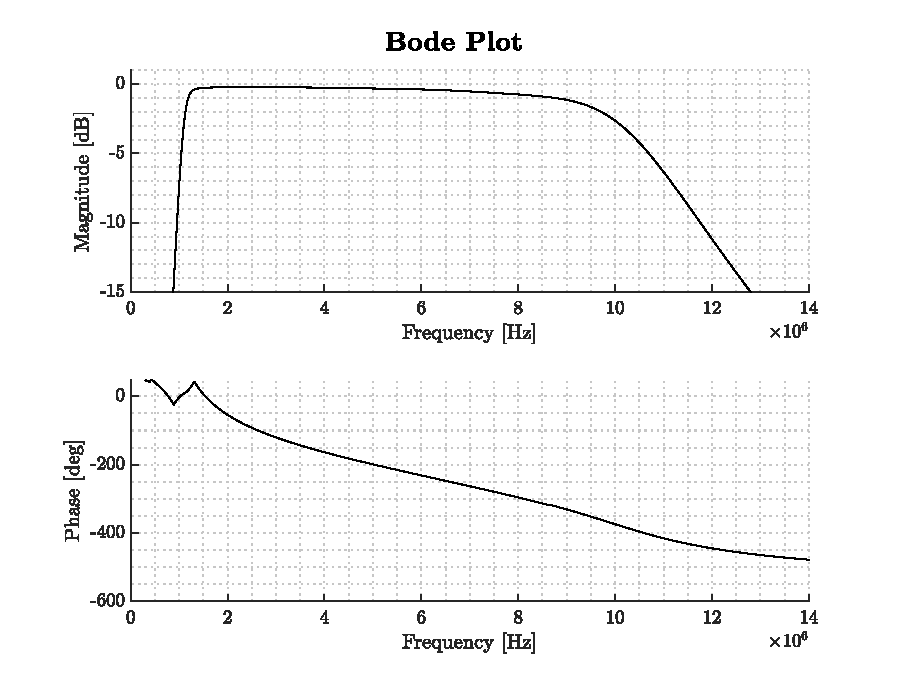
\includegraphics[width=.8\textwidth]{Figures/4_bpf_measurement_vna.eps}
	\caption[Band-pass filter bode plot]{Band-pass Filter bode plot from \qtyrange{0.3}{14}{\mega\hertz} with (above) magnitude and (below) phase}
	\label{fig:4_bpf_measurement}
\end{figure}

\subsection{Preamplifier}
Seen in \cref{fig:4_preamp_in} are measurements of the preamplifier circuits showing a \qty{70}{\milli\volt} input signal and a \qty{300}{\milli\volt} output signal with a \qty{2.5}{\volt} DC bias. In this application, however, only the \gls{lna} is used, and the \gls{vga} is bypassed in the hardware preamplifier configuration. The schematic of the preamplifier circuit is part of the demodulation schematic and can be found in the appendix in \cref{fig:appendix_ad8333}.
\begin{figure}[htbp]
	\centering
	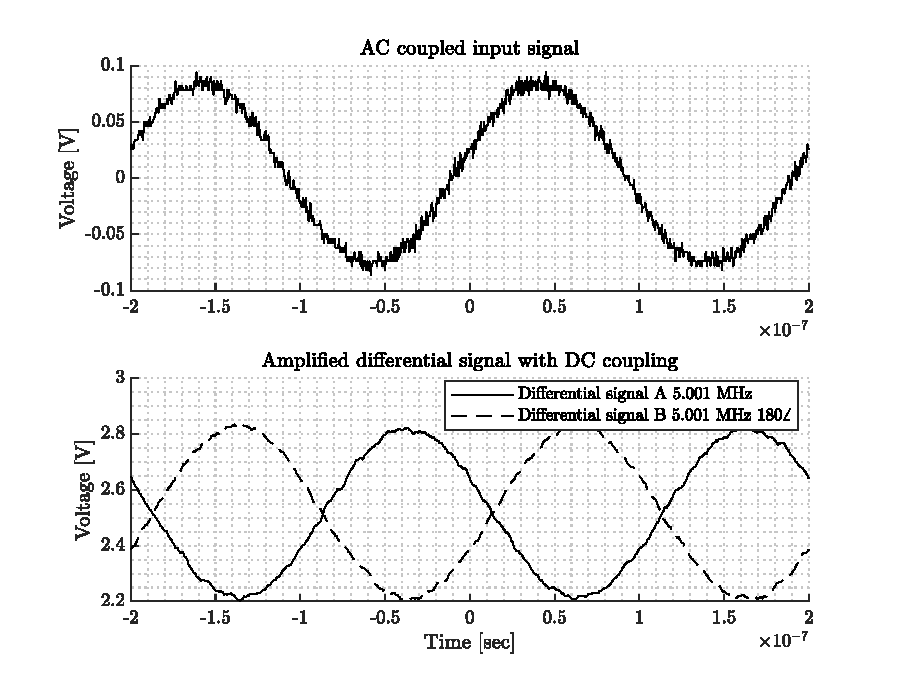
\includegraphics[width=.8\textwidth]{Figures/4_preamplifier_pcb.eps}
	\caption[Measured input and output of preamplifier PCB]{Measured input of preamplifier PCB, (Above) AC coupled input signal with amplitude \qty{1}{\volt} (Below Measured output of preamplifier PCB, Differential signal with DC coupling and $\times \qty{19}{\decibel}$ amplification)}
	\label{fig:4_preamp_in}
\end{figure}

\subsection{Demodulator}
Seen in \cref{fig:4_demod_in} are the input signals, differential signals of \qty{5.001}{\mega\hertz} and \qty{20}{\mega\hertz} local oscillator signal. Seen in \cref{fig:4_demod_out} are the differential input signals $A$ and $B$ and the demodulated output signals $I$ and $Q$, where the phase between $I$ and $Q$ denotes the Doppler shift direction, or rather, the direction of flow of the scatterer. It is noted that the differential signal is so high frequency compared to the timescale so there has to be a zoomed in subplot where the waveform is visible to show the waveform. This highlights the significant frequency difference, which is one of the key functions of the demodulator.

\begin{figure}[htbp]
	\centering
	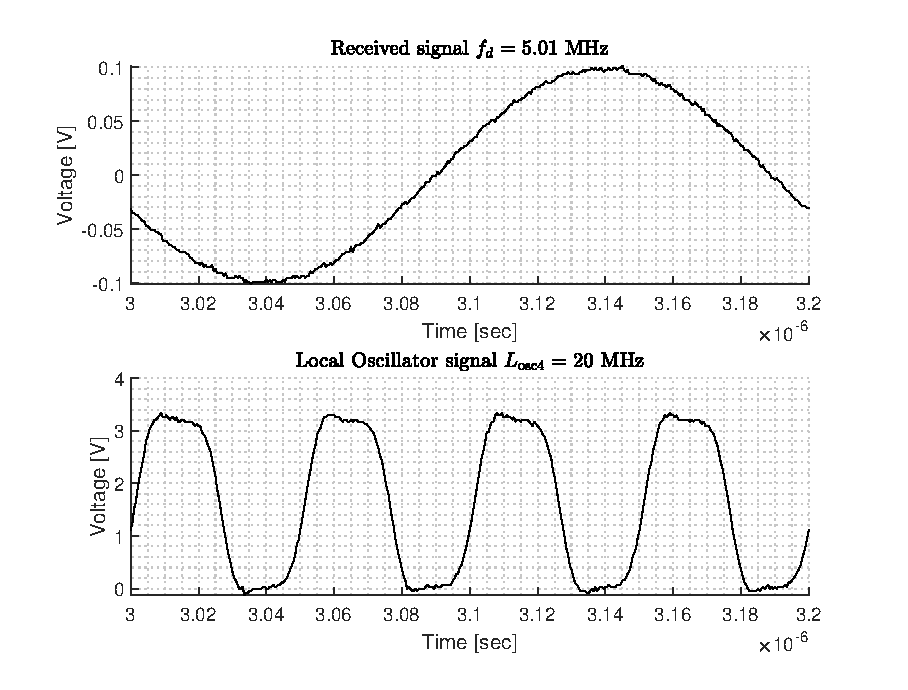
\includegraphics[width=.8\textwidth]{Figures/4_demod_pcb_in.eps}
	\caption[Measured input of demodulator PCB]{Measured input of demodulator PCB (Above) Input from received signal (Below) Input from local oscillator ($f_{0}\cdot4$)}
	\label{fig:4_demod_in}
\end{figure}
\begin{figure}[htbp]
	\centering
	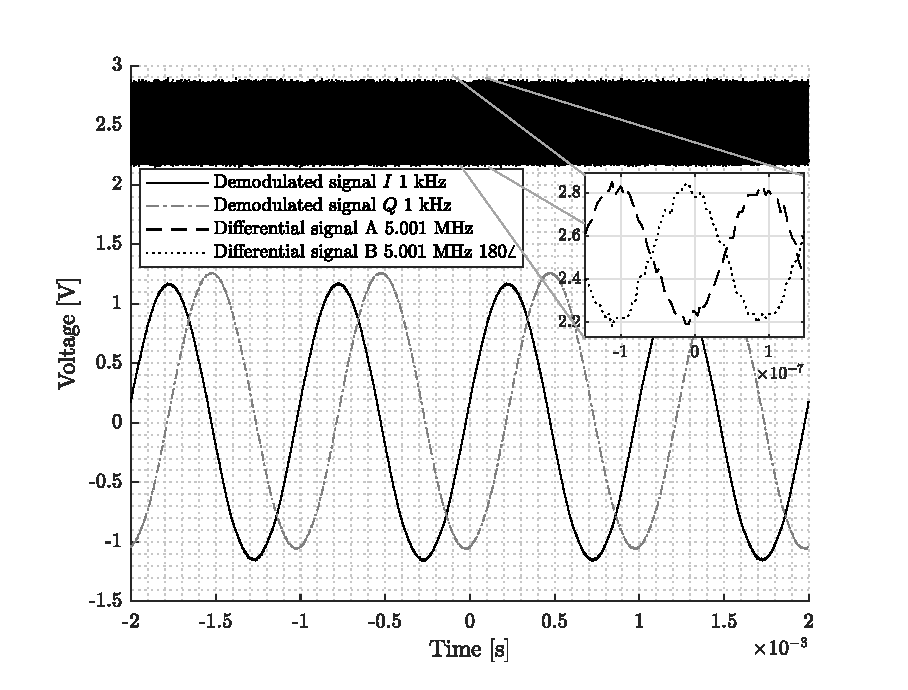
\includegraphics[width=.8\textwidth]{Figures/4_demod_pcb_out.eps}
	\caption[Measured output of demodulator PCB]{Measured output of demodulator PCB}
	\label{fig:4_demod_out}
\end{figure}

\subsection{Sample and Hold Amplifier}
Seen in \cref{fig:4_sample_hold_pcb} is the measured inputs and outputs of the circuit during the experiment. Above is the I-Q input and in the middle is the sample gating, and below is the output signal. On the output signal, it is noted the corresponding voltage transients for every pulse in the gate input.
\begin{figure}[htbp]
	\centering
	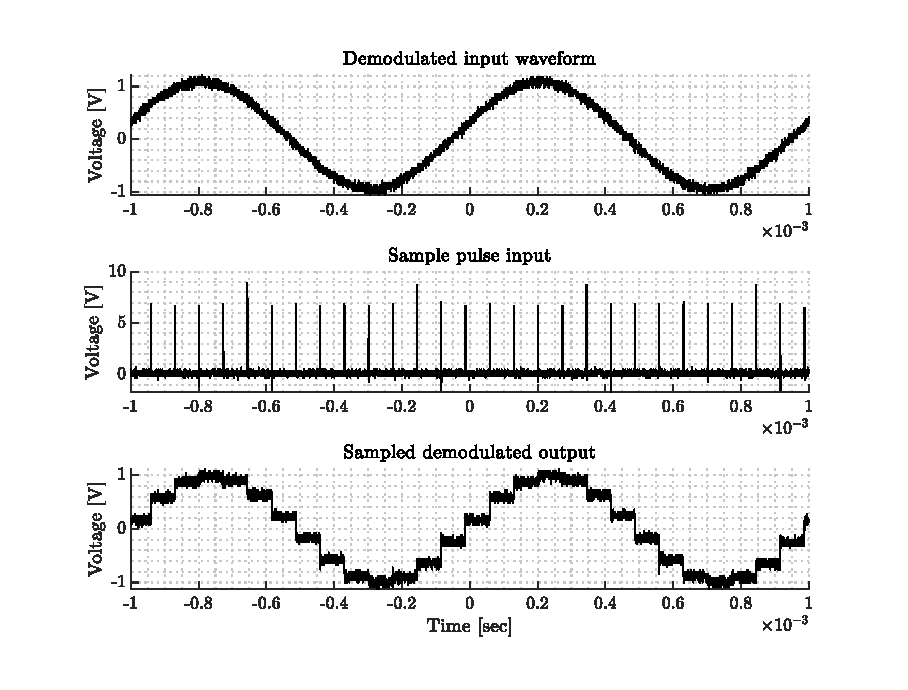
\includegraphics[width=.8\textwidth]{Figures/4_sampler_pcb.eps}
	\caption{Measured input and output of Sample and Hold amplifier}
	\label{fig:4_sample_hold_pcb}
\end{figure}

\subsection{Active Filter, DC Coupler}
\begin{align}
	\centering
	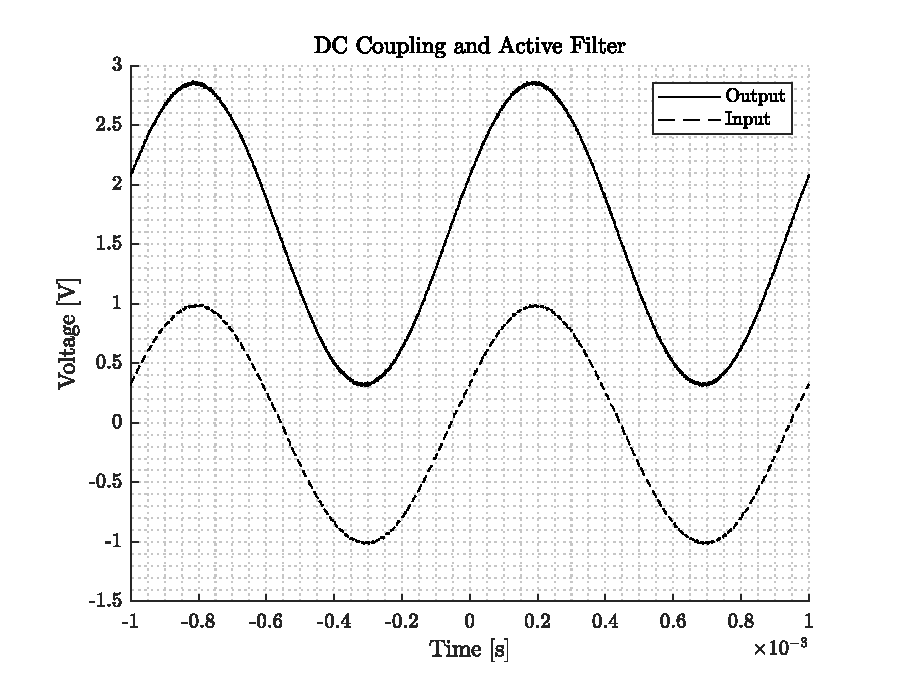
\includegraphics[width=.8\textwidth]{Figures/5_dccoupler_filter_measurement.eps}
	\caption{Measured input and output of Active filter and DC Coupler}
	\label{fig:5_dccoupler_measured}
\end{align}
Seen in \cref{fig:5_dccoupler_measured} is the measured input and output of the DC coupler and active filter. The dashed line is the \gls{ac} coupled input signal with \qty{1}{\volt} amplitude and the solid line is the amplified \gls{dc} coupled output signal.

\section{Pulse Generator and Power Stage}
Using the pulse generator and the power stage, an experiment is performed where the complementary PWM signals are generated and output to the gate driver of the power stage. In turn, the gate driver will drive the MOSFET pair and output a high-power output than the pulse generator can supply on its own through its GPIO.

\begin{figure}[htbp]
	\centering
	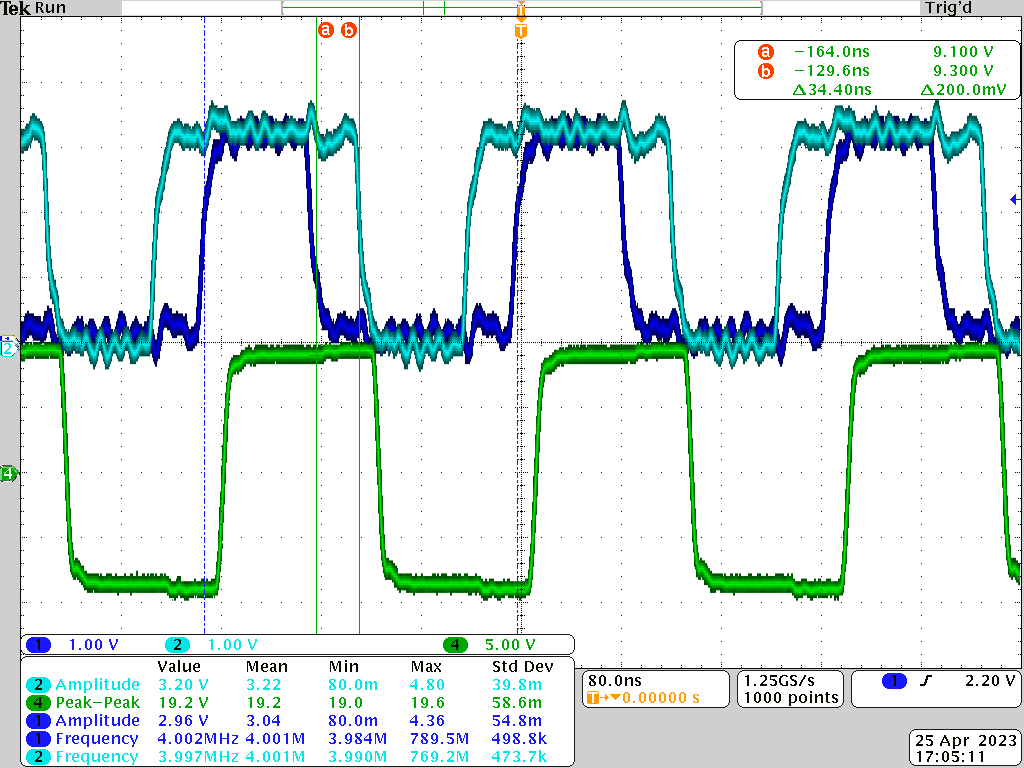
\includegraphics[width=.8\textwidth]{Figures/5_controlsystem_fpga_pwm.png}
	\caption{Complementary PWM output from the pulse generator and bipolar high power pulses}
	\label{fig:5_pulse_generator_experiment}
\end{figure}

Seen in \cref{fig:5_pulse_generator_experiment} are the measurements obtained from the pulse generator and power stage experiment. The measurements show the ability of the Pynq Z1 as a pulse generator is functioning as expected. As the power stage half-bridge is rail-to-rail, the output pulse voltages depend on the power supply voltage. In this case, the experiment is using a \qty{30}{\volt} maximum \gls{dcps}, and the output peak pulse voltages are $\pm \qty{30}{\volt}$. However, the power stage itself is specified for operating voltages up to $\pm \qty{100}{\volt}$.

\section{Doppler String Phantom Experiment}
The CIRS A043 Doppler String Phantom is a device used to evaluate the performance of Doppler ultrasound imaging systems. The phantom consists of a set of strings that move in a controlled manner when exposed to ultrasound waves. The strings are made of nylon monofilament and are arranged in a parallel array.

When the phantom is scanned with a Doppler ultrasound probe, the strings vibrate in response to the sound waves, producing a Doppler signal. The phantom includes a set of control strings that vibrate at a known frequency, allowing the user to calibrate the system and determine its accuracy. The string is driven by a motor that can be programmed to move at different speeds and directions, and it is also designed to create turbulence, which mimics the flow of blood in diseased vessels.

The phantom also includes a set of strings that move in a complex, non-linear pattern, simulating blood flow in vessels with turbulent flow. This allows the user to test the system's ability to accurately detect and measure turbulent blood flow, which is an important diagnostic feature for conditions such as stenosis or arterial occlusion.

By evaluating the system's performance on the known frequencies of the control strings and the complex patterns of the turbulence strings, the user can assess the accuracy and reliability of the Doppler ultrasound system. The CIRS A043 Doppler String Phantom is widely used in research, development, and quality assurance of Doppler ultrasound equipment.
\begin{figure}[htbp]
	\centering
	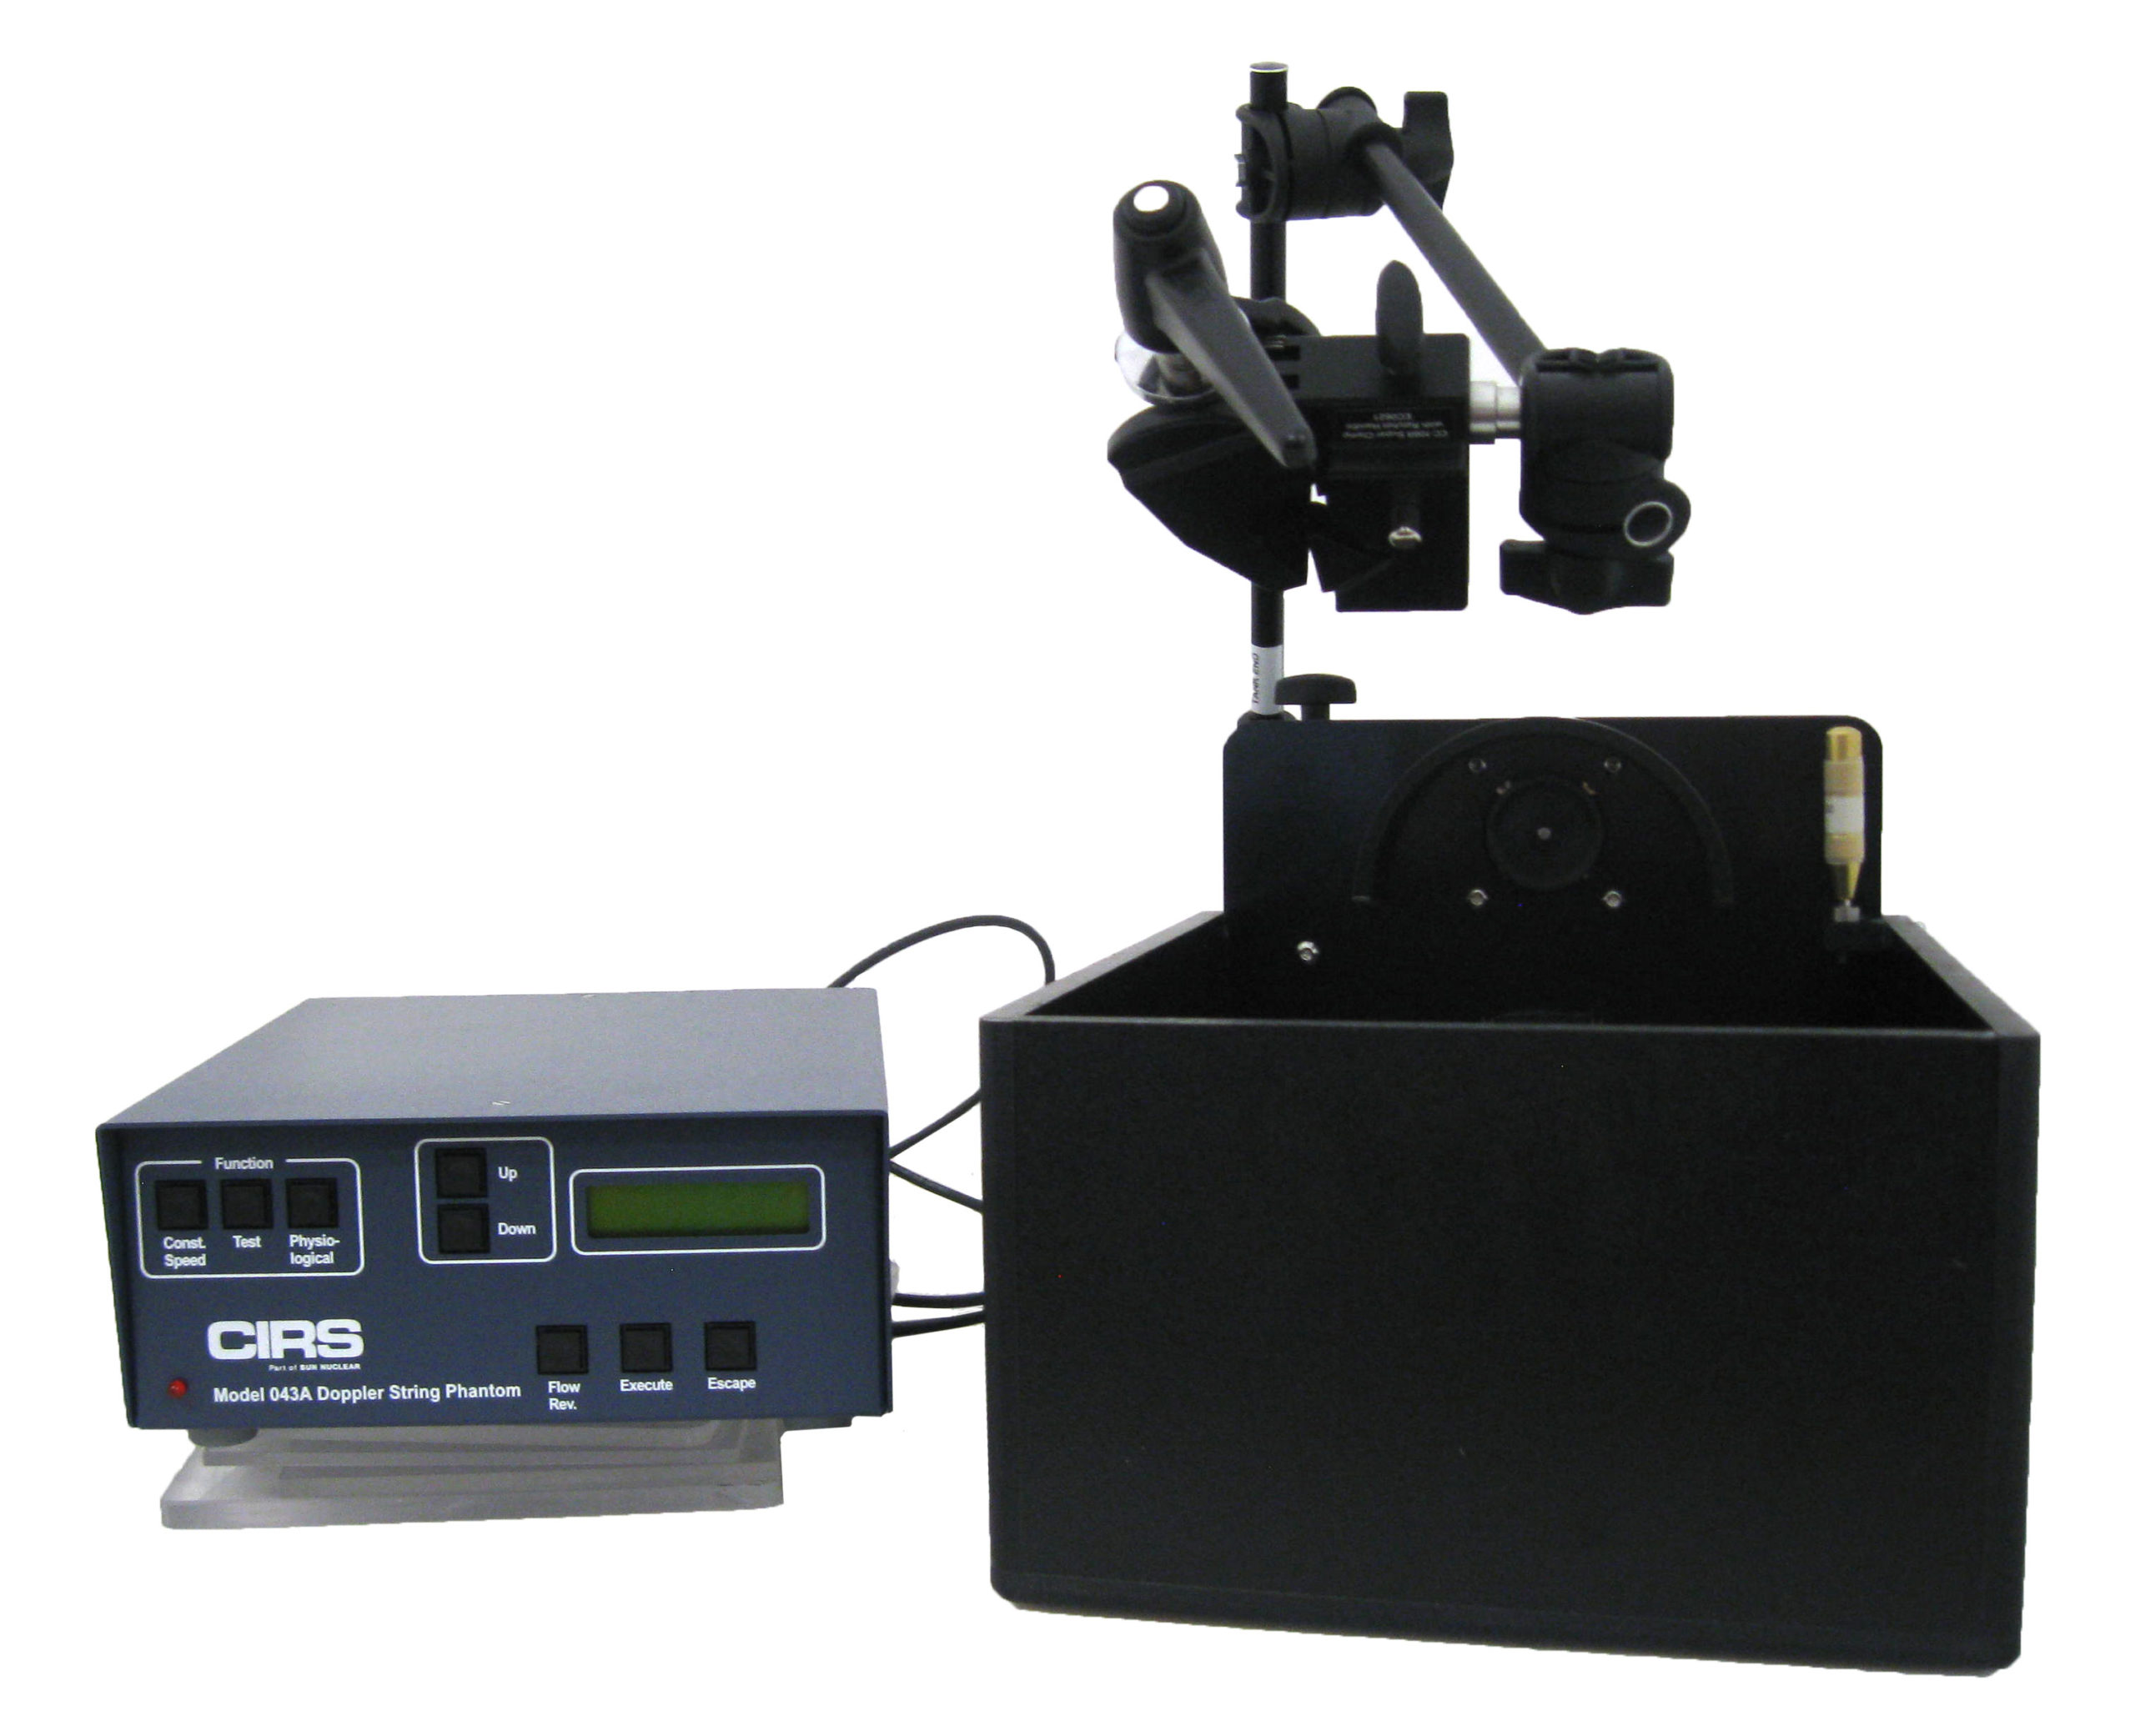
\includegraphics[width=.8\textwidth]{Figures/5_cirs_043a_image.jpg}
	\caption[CIRS Model 043A Doppler String Phantom]{CIRS Model 043A Doppler String Phantom with (left) motor controller and (right) tank and string loop}
\end{figure}

\begin{figure}[htbp]
	\centering
	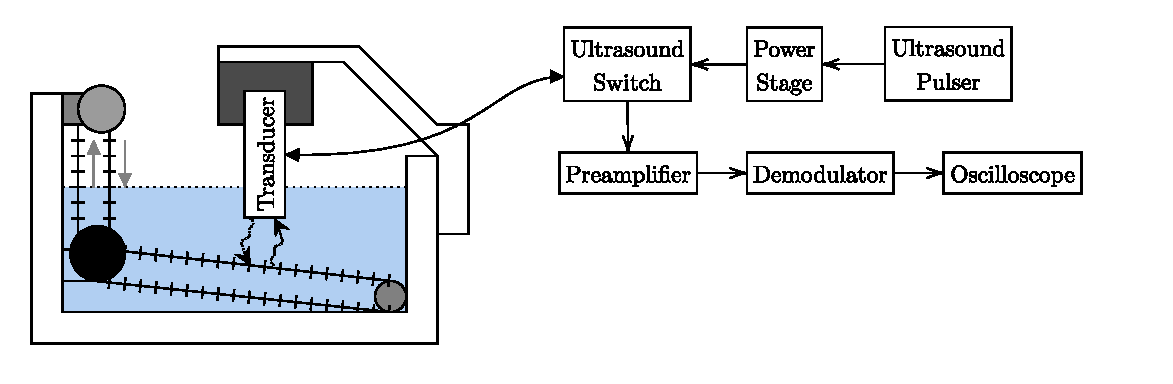
\includegraphics[width=.8\textwidth]{Figures/5_doppler_string_phantom_experiment.pdf}
	\caption{Doppler String Phantom experiment diagram (not to scale)}
	\label{fig:5_doppler_string_experiment}
\end{figure}

\pgfplotstableread{
x  {Name 1} {Name 2}    {Name 3}    {Name 4}
1  0.847    0.786       0.367       0.742
2  1.73     0.838       1.27        1.05
3  1.50     0.952       0           0
4  0.506    1.05        0.751       0.698
5  0.672    0.777       0           0
6  0.349    1.62        1.16        0.655
7  0.498    0.480       0.375       0.306
8  0.454    0.925       0.498       0.375
9  0.698    0.716       0.733       0.541
10 0.829    1.12        0.803       0.725
}\stackedColumnData

\begin{figure}[htb]
\centering
\begin{tikzpicture}
\begin{axis}[
    width=15cm, % You could use \linewidth instead
    height=6.6cm,
    ybar stacked,
    xtick = data,
    xticklabels={1,2,3,4,5,6,Var 1,Var 2,Var 3,Var 4},
    ylabel={Some text with a unit $\phi$ },
    ymajorgrids=true,
    legend style={at={(0.5,-0.1)}, anchor=north},
    cycle list name=DTU,
    every axis plot/.append style={fill,draw=none},
    ]
\addplot table[x=x,y={Name 1}]{\stackedColumnData};
\addplot table[x=x,y={Name 2}]{\stackedColumnData};
\addplot table[x=x,y={Name 3}]{\stackedColumnData};
\addplot table[x=x,y={Name 4}]{\stackedColumnData};
\legend{Heating,Ventilation,Lighting,Solar shading}
\end{axis}
\end{tikzpicture}
\caption{Stacked column chart}
\label{fig:stackedcolumn}
\end{figure}



\pgfplotstableread{
y {Name 1} {Name 2} {Name 3} {Name 4}
1 50        20      15       15
2 10        40      25       25
3 40        30      20       10
4 30        10      20       40
5 30        20      10       40
6 20        10      40       30
7 10        10      50       30
}\stackedBarData

\begin{figure}[H]%
\centering
\begin{tikzpicture}
\begin{axis}[
    width=15cm-10pt, % pgfplots widths are only approximate. You might have to fine tune the width of your figures to deal with overfull hbox warnings.
    height = 6.6cm,
    xbar stacked,
    xlabel=Write something here,
    ytick=data,
    yticklabels = {Text 1, Text 2, Text 3, Text 4, Text 5, Text 6, Text 7},
    xmin = 0,
    enlarge x limits=false,
    xmajorgrids=true,
    legend style={at={(0.5,-0.22)}},
    cycle list name=DTU,
    every axis plot/.append style={fill,draw=none},
    ]
\addplot table[x={Name 1},y=y]{\stackedBarData};
\addplot table[x={Name 2},y=y]{\stackedBarData};
\addplot table[x={Name 3},y=y]{\stackedBarData};
\addplot table[x={Name 4},y=y]{\stackedBarData};
\legend{Legend 1, Legend 2, Legend 3, Legend 4}
\end{axis}
\end{tikzpicture}
\caption{Stacked bar chart}
\label{fig:stackedbar}
\end{figure}



\pgfplotstableread{
x    {Far}  {Near}  {Here}
1930 50     38      15
1940 33     42      12
1950 40     43      13
1960 50     45      25
1970 70     65      35
}\groupedColumnData

\begin{figure}[H]
\centering
\begin{tikzpicture}
\begin{axis}[
    width=15cm,
    height=6.6cm,
    ybar,
    xtick=data,
    x tick label style={ /pgf/number format/1000 sep=},
    ylabel=Population,
    ymin=0,
    ymajorgrids=true,
    legend style={at={(0.5,-0.15)},anchor=north,legend columns=-1},
    cycle list name=DTU,
    ]
\addplot table[x=x,y={Far}]{\groupedColumnData};
\addplot table[x=x,y={Near}]{\groupedColumnData};
\addplot table[x=x,y={Here}]{\groupedColumnData};
\addplot[red,sharp plot,update limits=false] coordinates {(1910,43) (1990,43)} node[above] at (axis cs:1950,43) {Houses};
\legend{Far,Near,Here,Annot}
\end{axis}
\end{tikzpicture}
\caption{Grouped column chart}
\label{fig:groupedcolumn}
\end{figure}



\pgfplotstableread{
x {Name 1} {Name 2} {Name 3} {Name 4}
1 0         10       58       10
2 30        20       48       40
3 10        60       45       10.5
4 50        18       55       60
5 40        30       8        20
}\lineGraphData

\begin{figure}[H]
\centering
\begin{tikzpicture}[spy using outlines = {circle, size=2cm, magnification=5, connect spies}]
\begin{axis}[
    width=15cm,
    height=6.6cm,
    ylabel = {Unit},
    ymin = 0,
    enlarge x limits = false,
    ymajorgrids = true,
    legend style = {at={(0.5,-0.1)}, anchor=north},
    cycle list name=DTU,
    every axis plot/.append style={fill opacity=0},
    ]
\addplot table[x=x,y={Name 1}]{\lineGraphData};
\addplot table[x=x,y={Name 2}]{\lineGraphData};
\addplot table[x=x,y={Name 3}]{\lineGraphData};
\addplot table[x=x,y={Name 4}]{\lineGraphData};
\legend{Legend 1, Legend 2, Legend 3, Legend 4}
\end{axis}
\end{tikzpicture}
\caption{Line graph}
\label{fig:linegraph}
\end{figure}



\pgfplotstableread{
x {Name 1} {Name 2} {Name 3} {Name 4}
1 0         10       58       10
2 30        20       48       40
3 10        60       45       10.5
4 50        18       55       60
5 40        30       8        20
}\lineGraphMagnifyData

\begin{figure}[H]
\centering
\begin{tikzpicture}[spy using outlines = {circle, size=2cm, magnification=5, connect spies}]
\begin{axis}[
    width=15cm,
    height=6.6cm,
    ylabel = {Unit},
    ymin = 0,
    enlarge x limits = false,
    ymajorgrids = true,
    legend style = {at={(0.5,-0.1)}, anchor=north},
    cycle list name=DTU,
    every axis plot/.append style={fill opacity=0},
    ]
\addplot table[x=x,y={Name 1}]{\lineGraphMagnifyData};
\addplot table[x=x,y={Name 2}]{\lineGraphMagnifyData};
\addplot table[x=x,y={Name 3}]{\lineGraphMagnifyData};
\addplot table[x=x,y={Name 4}]{\lineGraphMagnifyData};

\coordinate (spypoint) at (axis cs:3,10.5); % Delete this line to remove magnifying glass
\coordinate (magnifyglass) at (axis cs:3.6,12); % Delete this line to remove magnifying glass
\legend{Legend 1, Legend 2, Legend 3, Legend 4}
\end{axis}

\spy [black, size=2cm] on (spypoint) in node[fill=white] at (magnifyglass); % Delete this line to remove magnifying glass
\end{tikzpicture}
\caption{Line graph with magnifying glass}
\label{fig:linegraphmagnify}
\end{figure}



\pgfplotstableread{
x {Name 1} {Name 2} {Name 3} {Name 4}
1 30        10       2        10
2 20        20       5        5
3 25        20       5        8
4 15        20       5        5
5 30        10       8        2
}\areaGraphData

\begin{figure}[H]
\centering
\begin{tikzpicture}
\begin{axis}[
    width=15cm,
    height=6.6cm,
    stack plots=y,
    area style,
    ylabel = {Unit},
    ymin = 0,
    enlarge x limits=false,
    ymajorgrids=true,
    legend style={at={(0.5,-0.1)}, anchor=north},
    cycle list name=DTU,
    ]
\addplot table[x=x,y={Name 1}]{\areaGraphData}\closedcycle;
\addplot table[x=x,y={Name 2}]{\areaGraphData}\closedcycle;
\addplot table[x=x,y={Name 3}]{\areaGraphData}\closedcycle;
\addplot table[x=x,y={Name 4}]{\areaGraphData}\closedcycle;
\legend{Legend 1, Legend 2, Legend 3, Legend 4}
\end{axis}
\end{tikzpicture}
\caption{Area graph}
\label{fig:areagraph}
\end{figure}



\pgfplotstableread{
x {Name 1} {Name 2} {Name 3} {Name 4}
1   11	15	38	41
2   33	22	25	31
3   22	25	11	21
4   44	14	17	51
5   13	42	25	33
6   14	52	36	34
}\scatterData

\begin{figure}[H]
\centering
\begin{tikzpicture}
\begin{axis}[
    %enlarge x limits=true,
    ylabel = {Unit},
    ymin = 0,
    ymajorgrids=true,
    cycle list name=DTU,
]
\addplot+[only marks,mark=*]        table[x=x,y={Name 1}]{\scatterData};
\addplot+[only marks,mark=square*]  table[x=x,y={Name 2}]{\scatterData};
\addplot+[only marks,mark=triangle*]table[x=x,y={Name 3}]{\scatterData};
\addplot+[only marks,mark=+]        table[x=x,y={Name 4}]{\scatterData};
\legend{Legend 1, Legend 2, Legend 3, Legend 4}
\end{axis}
\end{tikzpicture}
\caption{Scatter plot}
\label{fig:scatter}
\end{figure}


\begin{figure}[H]
\centering
\begin{tikzpicture}
\begin{axis}[
    boxplot/draw direction=y,
    xtick={1,2,3},
    xticklabels={Group A, Group B, Group C},
    x axis line style={opacity=0},
    enlarge y limits,
    ymajorgrids,
    cycle list name=DTU,
    every axis plot/.append style={semithick},
]
\addplot+[draw=black,
boxplot prepared={
lower whisker=42, lower quartile=45,
median=47,
upper quartile=47.5, upper whisker=48,
},
] coordinates {(0,40) (0,34) (0,56)};
\addplot+[draw=black,
boxplot prepared={
lower whisker=36, lower quartile=39,
median=40,
upper quartile=41, upper whisker=43,
},
] coordinates {};
\addplot+[draw=black,
boxplot prepared={
lower whisker=41, lower quartile=44,
median=45,
upper quartile=46, upper whisker=47,
},
] coordinates {(0,35) (0,55)};
\end{axis}
\end{tikzpicture}
\caption{Boxplot}
\label{fig:boxplot}
\end{figure}

\begin{figure}[H]
	\centering
	\begin{circuitikz}[american voltages]
		\draw
		(0,0) to [short, *-] (6,0)
		to [V, l_=$\mathrm{j}{\omega}_m \underline{\psi}^s_R$] (6,2)
		to [R, l_=$R_R$] (6,4)
		to [short, i_=$\underline{i}^s_R$] (5,4)
		(0,0) to [open, v^>=$\underline{u}^s_s$] (0,4)
		to [short, *- ,i=$\underline{i}^s_s$] (1,4)
		to [R, l=$R_s$] (3,4)
		to [L, l=$L_{\sigma}$] (5,4)
		to [short, i_=$\underline{i}^s_M$] (5,3)
		to [L, l_=$L_M$] (5,0);
	\end{circuitikz}
	\caption{The nodes short, V, R and L are presented here, but there a lot more}
	\label{fig:5-circ}
\end{figure}




\section{Tables and figures}

\begin{table}[H]
\centering
\caption{This is a \texttt{booktabs} table}
\label{tab:tableExample}
\begin{tabular}{@{}llS@{}}
\toprule
Animal     & Description & {Price (\$)} \\ \midrule
Gnat       & per gram    & 13.65      \\
           & each        & 0.01       \\
Gnu        & stuffed     & 92.50      \\
Emu        & stuffed     & 33.33      \\
Armadillo  & frozen      & 8.99       \\ \bottomrule
\end{tabular}
\end{table}
\texttt{Booktabs} tables don't use any vertical lines. Only horizontal lines are used. \Cref{tab:tableExample} begins with a \textbackslash \texttt{toprule}, ends with a \textbackslash \texttt{bottomrule} with \textbackslash \texttt{midrule} in between. The table has 3 columns formatted as \texttt{@\{\}llS@\{\}}. \texttt{@\{\}} is cropping the horizontal lines of the table to fit the content (removes column spacing at the left and right edges). \texttt{l} aligns the column to the left and \texttt{S} aligns the column according to the decimal point (\texttt{siunitx} package). You can of course also use \texttt{r} to align right or \texttt{c} to center the contents of the column.

\begin{table}[H]
\centering
\caption{Wrongly formatted table}
\label{tab:tableExampleWrong}
\begin{tabular}{llll}
\toprule
                    & Voltage & Current   & Power   \\
                    & V       & A         & W       \\ \midrule
Transformer input   & 234.4   & 0.50      & 117.4   \\ \midrule
Transformer output  & 25.86   & 2.72      & 70.3    \\ \midrule
Efficiency          &         &           & 60\%    \\ \bottomrule
\end{tabular}
\end{table}

\begin{table}[H]
\centering
\caption{Correctly formatted table}
\label{tab:tableExampleCorrect}
\begin{tabular}{@{}lSSS@{}}
\toprule
                    & {Voltage} & {Current} & {Power}       \\
                    & V         & A         & W             \\ \midrule
Transformer input   & 234.4     & 0.50      & 117.4         \\
Transformer output  & 25.86     & 2.72      & 70.3          \\ \midrule
Efficiency          &           &           & \SI{60}{\percent} \\ \bottomrule
\end{tabular}
\end{table}

\Cref{tab:tableExampleWrong} and \cref{tab:tableExampleCorrect} have the same comtents but there are some subtle differences in formatting which makes \cref{tab:tableExampleCorrect} the superior table of the two. The most obvious change is removing the midrule between the transformer input and output rows. The efficency row is the odd man out and a midrule has been used to emphasise the difference between the transformer rows and the efficiency row. The delimiters in the voltage, current and power columns are aligned. The horizontal lines (rules) fits to the content and instead of protruding. The spacing between 60 and the percentage sign is correctly adjusted.

\begin{figure}[H]
\centering

\includegraphics[width=0.3\textwidth]{Pictures/Logos/dtured_cmyk.pdf}
\caption{Just a normal figure}
\label{fig:figure}
\end{figure}

\begin{figure}[H]
\centering
\begin{subfigure}{.5\textwidth}
  \centering
  
\includegraphics[width=.4\linewidth]{Pictures/Logos/dtured_cmyk.pdf}
  \caption{A subfigure}
  \label{fig:twosub1}
\end{subfigure}%
\begin{subfigure}{.5\textwidth}
  \centering
  
\includegraphics[width=.4\linewidth]{Pictures/Logos/black_cmyk.pdf}
  \caption{A subfigure}
  \label{fig:twosub2}
\end{subfigure}
\caption{A figure with two subfigures}
\label{fig:twosubfigures}
\end{figure}

\begin{figure}[H]
\centering
\begin{subfigure}{.49\textwidth}
  \centering
  
\includegraphics[width=.3\linewidth]{Pictures/Logos/dtured_cmyk.pdf}
  \caption{A subfigure}
  \label{fig:foursub1}
\end{subfigure}%
\begin{subfigure}{.49\textwidth}
  \centering
  
\includegraphics[width=.3\linewidth]{Pictures/Logos/black_cmyk.pdf}
  \caption{A subfigure}
  \label{fig:foursub2}
\end{subfigure}
\begin{subfigure}{.49\textwidth}
  \centering
  
\includegraphics[width=.3\linewidth]{Pictures/Logos/black_cmyk.pdf}
  \caption{A subfigure}
  \label{fig:foursub3}
\end{subfigure}
\begin{subfigure}{.49\textwidth}
  \centering
  
\includegraphics[width=.3\linewidth]{Pictures/Logos/dtured_cmyk.pdf}
  \caption{A subfigure}
  \label{fig:foursub4}
\end{subfigure}
\caption{A figure with four subfigures}
\label{fig:foursubfigures}
\end{figure}

Referring to the figure as a whole \cref{fig:foursubfigures} or to an individual sub figure \cref{fig:foursub1} is done the normal way with \texttt{\textbackslash cref\{\}} commands.


\section{Equations}
In-line math is easy. Anything surrounded by dollar signs becomes a math field. Here is an example: $f(x)=2x-1$. Also anything inside the ``\textbackslash begin\{equation\}'' and  ``\textbackslash end\{equation\}'' environment is also a math field. Examples are shown below.

All equations use the default latex font. Some might say it looks weird with a serif font for equations and a sans-serif font for the body text. However, it is very unpractical to change the math font in latex which is the exactly the reason why this has not been done. One benefit of the serif style math font is the clear distinction between symbols (variables) and units.

On the subject of units, those are all taken care of by the \texttt{\textbackslash siunitx} package. Whenever there is a number followed by a unit one should write \textbackslash SI\{number\}\{unit\}. Note this command is case sensitive. If a unit should follow a variable use the command \textbackslash si\{unit\} (also case sensitive).

The ideal gas law is shown in \cref{eq:idealgaslaw}.
\begin{equation} \label{eq:idealgaslaw}
    p \cdot V = n \cdot R \cdot T
\end{equation}

\begin{equation} \label{eq:IME}
    \frac{\partial}{\partial t} \int_{0}^{\delta} U dy = - \delta \frac{1}{\rho}\frac{\partial P}{\partial x}-U_f(t)^2
\end{equation}

\begin{equation} \label{eq:penDepthStep}
d_{step} = \sqrt{\frac{\delta}{\frac{dw}{dp_v}} \cdot t} =
\sqrt{\frac{\SI{1.0e-11}{kg/(m.s.Pa)}}{\frac{\SI{5.4}{kg/m^3}}{\SI{233.82}{Pa}}} \cdot \SI{7200}{s}} =
\SI{0.001766}{m} = \SI{1.766}{mm}
\end{equation}

\begin{equation} \label{eq:equilibrium}
\begin{aligned}
    CH_3COOH + OH^{-} &\rightleftharpoons CH_3COO^{-} + H_2O \\
    H_2O &\rightleftharpoons H^{+}_{(aq)} + OH^{-}_{(aq)}
\end{aligned}
\end{equation}


\begin{align}
    \label{eq:align1}
    f(x) &= 1 + x - 3 x^2 \\
    \label{eq:align2}
    g(x) + y &= 3x - \frac{1}{2} x^3
\end{align}
